\documentclass{article}
\usepackage{graphicx}
\usepackage{wrapfig}
\usepackage{filecontents}
\usepackage{siunitx}
\usepackage[table]{xcolor}
\usepackage{float}
\usepackage{hyperref}
\usepackage{color} % balíček pro obarvování textů
\usepackage{xcolor}  % zapne možnost používání barev, mj. pro \definecolor
\hypersetup{
    colorlinks,
    linkcolor={red!50!black},
    citecolor={green!50!black},
    urlcolor={blue!80!black}
}
\definecolor{orange}{RGB}{   251,	 114,	 32}

\usepackage[total={175mm,230mm}, top=23mm, left=20mm, includefoot]{geometry}
\usepackage{pgfplots}
\usepackage{blindtext}

\usepackage{subfiles} % Best loaded last in the preamble

\usepackage{bookmark}

\begin{document}
\begin{figure}[H]
    \centering
    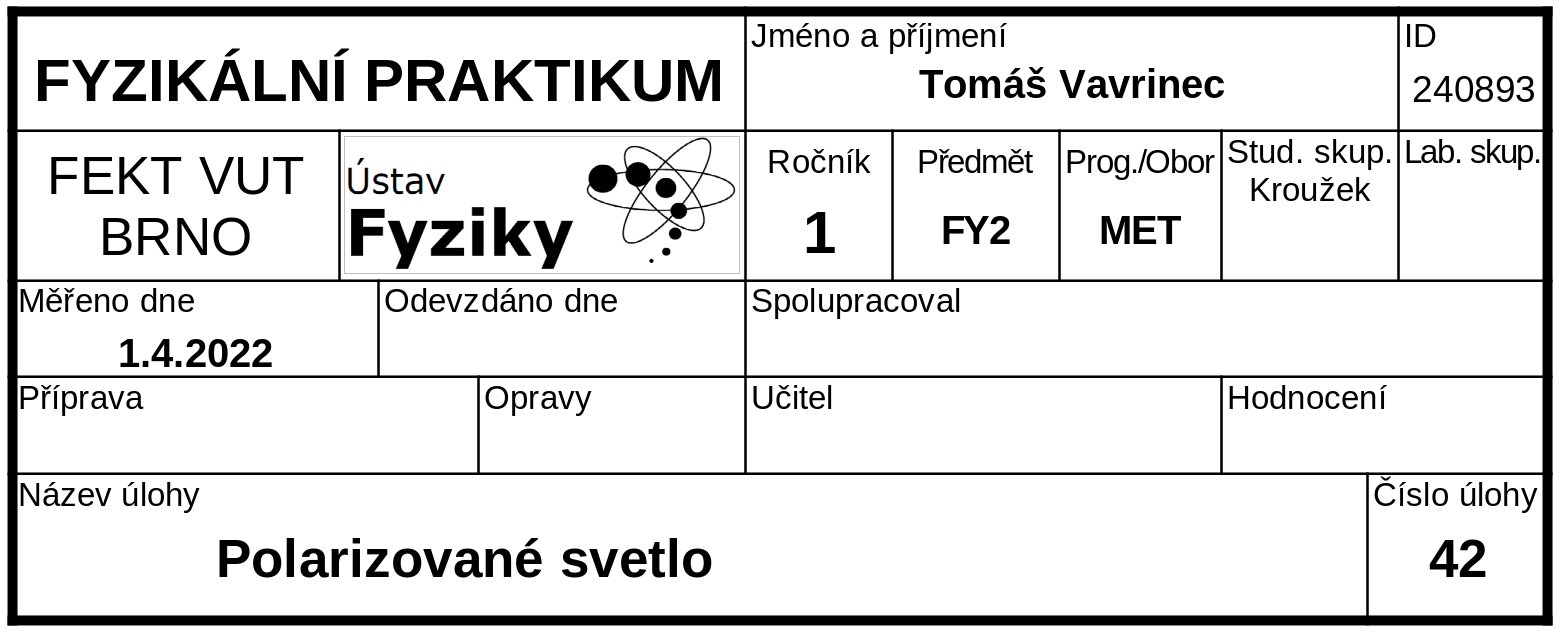
\includegraphics[width=0.9\textwidth]{hlavička.png}
\end{figure}

\small
\section{Úkol}
\begin{enumerate}
    \item Ověřte platnost Malusova zákona.
    \item Změřte Brewsterův úhel a nalezněte relativní index lomu dvou prostředí.
\end{enumerate}

\section{Teoretický úvod}
Elektromagnetické vlnění se skládá z elektrické \overrightarrow{E} a magnetické \overrightarrow{B} složky.
Obě složky jsou vždy navzájem kolmé a zároveň kolmé k vektoru šíření, kolem kterého se mohou během šíření otáčet.
Pokud toto otáčení není náhodné, nazývá se tento jev polarizace.

Díky provázání obou složek popsanými Maxwellovými rovnicemi se pro popis elektromagnetické vlny dá použít jen jedna ze složek.
Polarizace se proto popisuje pomocí elektrické složky.

Popišme šířící se elektromagnetickou vlnu jako dvě na sebe kolmé sinusové složky šířící se po ose \(X\), přičemž jejich součet bude vyjadřovat vektor elektrické složky \overrightarrow{E}.
Můžeme rozdělit polarizaci na příčnou a eliptickou, jejímž speciálním případem je polarizace kruhová.
Příčně polarizovanou vlnu můžeme popsat pomocí dvou na sebe kolmých sinusoid, z nichž má jedna nulovou amplitudu.
Vektor elektrické složky tak kmitá v ploše.

Pomocí polarizátoru můžeme z nepolarizovaného světla vyrobit světlo polarizované, u kterého pak pomocí dalšího polarizátoru lze určit směr polarizace.
\subsection*{Polarizace průchodem - Malusův zákon}
Z lineárně polarizovaného světla dopadající na lineární polarizátor projde jen složka rovnoběžná s polarizační rovinou polarizátoru.
Platí
\begin{equation}
    I_p=L_0\cos{\alpha}^2
    \label{malus}
\end{equation}
Kde \(I_p\) je intenzita průchozího světla, \(I_0\) je intenzita dopadajícího světla a \(\alpha\) je úhel, který svírá polarizační rovinou polarizátoru s rovinou, ve které kmitá vektor elektrické intenzity \overrightarrow{e}.

\subsection*{Polarizace odrazem - Brewsterův úhel}
Při odrazu elektrické vlny od průhledného, homogeního a izotropního prostředí dochází k částečné polarizaci.
Pokud paprsek dopadá pod tzv. Brewsterovim úhlem \(\varphi_B\), odrazí se pouze část světla polarizovaného v rovině kolmé na rovinu, v niž leží trajektorie dopadajícího a odraženého paprsku.
Brewsterovým úhlem \(\varphi_B\) se také nazývá polarizační uhel. 
Jde o úhel mezi odraženým paprskem a normálou rozhraní v momentě, kdy je mezi odraženým a prošlým paprskem \(90^\circ\).
Platí tedy
\begin{equation}
    \varphi_B=\arctan{\frac{n_2}{n_1}}
    \label{brews}
\end{equation}
Kde \(n_1\) je index lomu prostředí, z něhož paprsek dopadá na prostředí s indexem lomu \(n_2\).

\section{Měření}
\subsection*{Malusův zákon}
Protože jako zdroj světla používáme laser s kruhovou polarizací, použijeme polarizátor, který nám vytvoříme lineárně polarizované světlo.
Dalším polarizátorem budeme otáčet, a tak měnit množství světla, které projde do detektoru.

\begin{figure}[H]
	\begin{minipage}[t]{0.35\textwidth}
        \paragraph*{Malusův\;zákon}
        \vspace*{-100mm}
        \begin{tabular}{|c|c|c|}
            \hline
            \(\alpha\)              & \(\delta_1\)                  & \(U_1\)                   \\ \hline
            \(\alpha_0 = 0^\circ\)  & \(\delta_0 = 110\;[^\circ]\)  & \(U_{max} = 5.06\;[V]\)   \\ \hline
            \(10^\circ\)            & 100                           & 3.8                       \\ \hline
            \(20^\circ\)            & 90                            & 2.5                       \\ \hline
            \(30^\circ\)            & 80                            & 1.5                       \\ \hline
            \(40^\circ\)            & 70                            & 0.6                       \\ \hline
            \(50^\circ\)            & 60                            & 0.133                     \\ \hline
            \(60^\circ\)            & 50                            & 0.014                     \\ \hline
            \(70^\circ\)            & 40                            & 0.383                     \\ \hline
            \(80^\circ\)            & 30                            & 1.1                       \\ \hline
            \(90^\circ\)            & 20                            & 1.9                       \\ \hline
                                                                                                   \hline
            \(\alpha\)              & \(\delta_2\)                  & \(U_2\)                   \\ \hline
            \(\alpha_0 = 0^\circ\)  & \(\delta_0 = 110\;[^\circ]\)  & \(U_{max} = 5.06\;[V]\)   \\ \hline
            \(10^\circ\)            & 120                           & 5.5                       \\ \hline
            \(20^\circ\)            & 130                           & 6.5                       \\ \hline
            \(30^\circ\)            & 140                           & 6.3                       \\ \hline
            \(40^\circ\)            & 150                           & 6.1                       \\ \hline
            \(50^\circ\)            & 160                           & 6.3                       \\ \hline
            \(60^\circ\)            & 170                           & 5.6                       \\ \hline
            \(70^\circ\)            & 180                           & 4.5                       \\ \hline
            \(80^\circ\)            & 190                           & 2.8                       \\ \hline
            \(90^\circ\)            & 200                           & 2.0                       \\ \hline
        \end{tabular}
    \end{minipage}
    \hfill
	\begin{minipage}[t]{0.57\textwidth}
        \pgfplotsset{width=110mm,compat=1.9}
        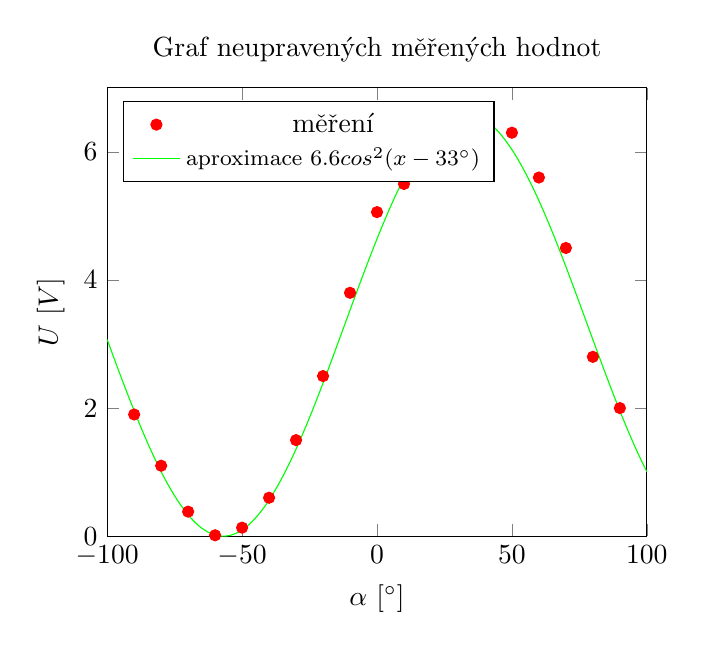
\begin{tikzpicture}
            \begin{axis}[
                % colorbar,
                title={Graf neupravených měřených hodnot},
                xlabel={\(\alpha~[^\circ]\)},
                ylabel={\(U~[V]\)},
                xmin=-100, xmax=100,
                ymin=0, ymax=7,
                legend pos=north west,
            ]
            \addplot[
                only marks,
                color=red,
                mark=*,
                ]
                coordinates {
                    (90 , 2.0  )
                    (80 , 2.8  )
                    (70 , 4.5  )
                    (60 , 5.6  )
                    (50 , 6.3  )
                    (40 , 6.1  )
                    (30 , 6.3  )
                    (20 , 6.5  )
                    (10 , 5.5  )
                    (0  , 5.06 )
                    (-10, 3.8  )
                    (-20, 2.5  )
                    (-30, 1.5  )
                    (-40, 0.6  )
                    (-50, 0.133)
                    (-60, 0.014)
                    (-70, 0.383)
                    (-80, 1.1  )
                    (-90, 1.9  )
                    };
                \addlegendentry{měření}
            \addplot[
                color = green,
                domain=-100:100,
                samples=500,
                ]
                    {6.6*cos(x-33)*cos(x-33)};
                \addlegendentry{\footnotesize{aproximace \(6.6cos^2(x-33^\circ)\)}}
            \end{axis}
        \end{tikzpicture}
    \end{minipage}
\end{figure}
\begin{figure}[H]
    \hspace{-5mm}
	\begin{minipage}[t]{0.5\textwidth}
        \pgfplotsset{width=100mm,compat=1.9}
        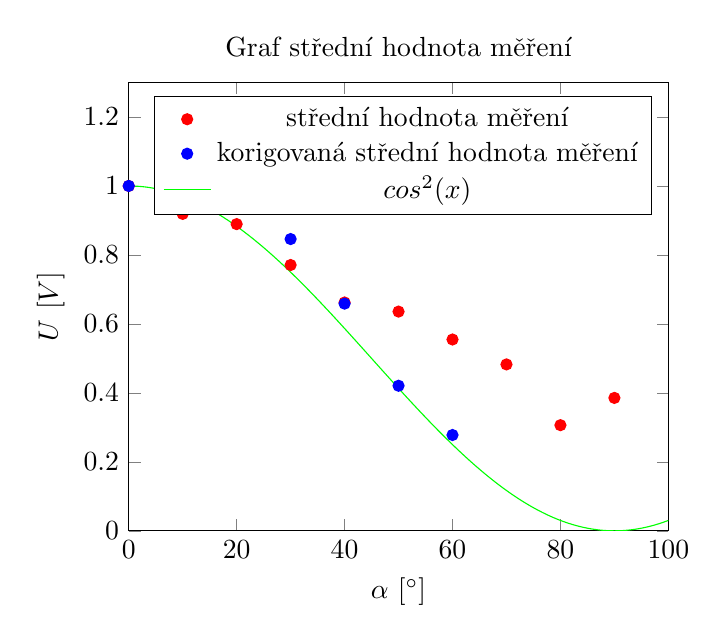
\begin{tikzpicture}
            \begin{axis}[
                title={Graf střední hodnota měření},
                xlabel={\(\alpha~[^\circ]\)},
                ylabel={\(U~[V]\)\hspace{-30mm}},
                xmin=0, xmax=100,
                ymin=0, ymax=1.3,
                legend pos=north east,
            ]
            \addplot[
                only marks,
                color=red,
                mark=*,
                ]
                coordinates {
                    (90, 1.95  /5.06)
                    (80, 1.55  /5.06)
                    (70, 2.4415/5.06)
                    (60, 2.807 /5.06)
                    (50, 3.2165/5.06)
                    (40, 3.35  /5.06)
                    (30, 3.9   /5.06)
                    (20, 4.5   /5.06)
                    (10, 4.65  /5.06)
                    (0 , 5.06  /5.06)
                    };
                \addlegendentry{střední hodnota měření}
            \addplot[
                only marks,
                color=blue,
                mark=*,
                ]
                coordinates {
                    ( 60, 1.75/6.3)
                    ( 50, 2.65/6.3)
                    ( 40, 4.15/6.3)
                    ( 30, 5.33/6.3)
                    ( 20, 5.9 /6.3)
                    ( 10, 6.3 /6.3)
                    (  0, 6.3 /6.3)
                    };
                \addlegendentry{korigovaná střední hodnota měření}
            \addplot[
                color = green,
                domain=-100:100,
                samples=500,
                ]
                    {(cos(x)*(cos(x)))};
                \addlegendentry{\(cos^2(x)\)}
            \end{axis}
        \end{tikzpicture}
    \end{minipage}
    \hfill
    \hspace{23mm}
	\begin{minipage}[t]{0.4\textwidth}
        \vspace{-80mm}
        Během našeho určování \(U_{max}\) se pravděpodobně změnila světelnost v~místnosti, což vedlo ke změně měřeného napětí. 
        Z toho důvodu jsme \(U_{max}\) určili chybně (výsledek je v grafu znázorněn červeně).
        Z grafu surového měření je vidět, že měření kopíruje cosinusoidu, ale posunutou o \(33^\circ\).
        
        Považujme proto bod \([6.3\;V; 30^\circ]\) za nové maximum a berme v úvahu jen šest měření v jeho okolí (výsledek je grafu znázorněn modře). 
    \end{minipage}
\end{figure}


\newpage
\subsection*{Brewsterův úhel}
Polarizátorem zajistíme světlo polarizované v rovině dopadu na rotující PMMA (PolyMethylMethAkrylát).
Protože PMMA rotuje uvnitř válcového stínítka, vytvoří odraženým světlem na jeho stěnách stopu.
Zároveň je lineárně polarizované v rovině dopadu, a tak se při dopadu pod Brewsterůvým úhlem \(\varphi_B\) neodrazí \(\Rightarrow\), stopa na stínítku bude na dvou místech přerušena.
Přerušení stopy nastane právě při hodnotě Brewsterova úhlu \(\varphi_B\), čehož využijeme pro jeho měření.

\begin{figure}[H]
	\begin{minipage}[t]{0.45\textwidth}
        \vspace{-85mm}
        \begin{tabular}{|c|c|c||c|c|c|}
            \hline
            \(\beta_{det}\)   & \(\varphi = \beta_{det}\)   & \(U\)     & \(\beta_{det}\)   & \(\varphi = \beta_{det}\)   & \(U\)       \\ \hline
            \([^\circ]\)      & \([^\circ]\)                & \([mV]\)  & \([^\circ]\)      & \([^\circ]\)                & \([mV]\)    \\ \hline
            160.2             & 80.1                        & 20.0      & 101.7             & 50.85                       & 1.7         \\ \hline
            155.7             & 77.85                       & 18.0      & 88.2              & 44.1                        & 2.2         \\ \hline
            151.2             & 75.6                        & 16.2      & 61.2              & 30.6                        & 2.5         \\ \hline
            146.7             & 73.35                       & 12.4      & 70.2              & 35.1                        & 2.9         \\ \hline
            142.2             & 71.1                        & 8.4       & 61.2              & 30.6                        & 3.3         \\ \hline
            128.7             & 64.35                       & 3.2       & 52.2              & 26.1                        & 3.8         \\ \hline
            119.7             & 59.85                       & 1.9       & 43.2              & 21.6                        & 4           \\ \hline
            110.7             & 55.35                       & 1.6       & 29.7              & 14.85                       & 6           \\ \hline
        \end{tabular}
        \begin{figure}
            Z měření plyne, že Brewsterův úhel \(\varphi_B\) je blízko \(55.35^\circ\), předpokládejme tedy \(\varphi_B = 55.35^\circ\)
            Pomocí Brewsterova úhlu \(\varphi_B\) určíme relativní index lomu ze vztahu \ref{brews} jako
            \\\\
            \large{
            \(
                \frac{n_2}{n_1} = \tan{\varphi_B} = \tan{55.35^\circ} = 1.45\;[-]
            \)
            }
        \end{figure}
    \end{minipage}
    \hfill
	\begin{minipage}[t]{0.5\textwidth}
        \pgfplotsset{width=100mm,compat=1.9}
        \tikzset{
        every pin/.style={fill=yellow!50!white,rectangle,rounded corners=3pt,font=\scriptsize},
        small dot/.style={fill=black,circle,scale=0.3}
        % /dotted
        }
        \begin{tikzpicture}
            \begin{axis}[
                % colorbar,
                title={Graf neupravených měřených hodnot},
                xlabel={\(\alpha~[^\circ]\)},
                ylabel={\(U~[V]\)\hspace{-30mm}},
                xmin=0, xmax=90,
                ymin=0, ymax=21,
                legend pos=north west,
            ]
            \addplot[
                only marks,
                color=green,
                mark=*,
                ]
                coordinates {
                    (80.1 , 20.0)
                    (77.85, 18.0)
                    (75.6 , 16.2)
                    (73.35, 12.4)
                    (71.1 , 8.4 )
                    (64.35, 3.2 )
                    (59.85, 1.9 )
                    (55.35, 1.6 ) %
                    (50.85, 1.7 )
                    (44.1 , 2.2 )
                    (30.6 , 2.5 )
                    (35.1 , 2.9 )
                    (30.6 , 3.3 )
                    (26.1 , 3.8 )
                    (21.6 , 4   )
                    (14.85, 6   )
                    };
                \addlegendentry{měření}
            \addplot[
                only marks,
                color=red,
                mark=*,
                ]
                coordinates {
                    (30.6 , 2.5 )
                    (21.6 , 4   )
                    };
                \addlegendentry{chybná měření}
            \addplot[
                only marks,
                color=orange,
                mark=*,
                ]
                coordinates {
                    (55.35, 1.6 )
                    };
                \addlegendentry{minimum měření}
            \node[small dot,pin=90:{\texttt{\([55.35^\circ;1.6\;V]\)}}] at (axis description cs:0.615,0.07619) {};
            \end{axis}
        \end{tikzpicture}
    \end{minipage}
\end{figure}
Protože paprsek dopadal na PMMA ze vzduchu, můžeme říct \(n_1 = 1\;[-]\), a tím pádem index lomu PMMA \(n_2 = 1.45\;[-]\)

\section{Závěr}
Kvůli chybě při určování maxima \(U_{max}\) při přípravě měření Malusova zákona mi graf znázorňující střední napětí při daném úhlu \(\alpha\) nevyšel a cosinusoidě se podobal jen klesavou tendencí.
Stanovil jsem proto nové maximum \(U_{max}\), což výsledky k cosinusoidě zásadně přiblížilo.

Brewsterův úhel jsem z měření stanovil na \(55.35^\circ\) a z něj určil index lomu PMMA jako \(n_2 = 1.45\), což znamená odchylku \(0.03\) od hodnoty \(n_2 = 1.48\), která je uvedena v zadání měření. 

\end{document}
